\chapter{页表}\label{ch03}

页表是最流行的帮助操作系统为每个进程提供私有地址空间和内存的机制。
页表决定了内存地址的含义和哪些物理内存可以被进程访问。
这允许xv6隔离开不同进程的地址空间并复用同一个物理内存。
页表是一个很流行的设计,因为它们提供了一个间接层,操作系统可以利用这个间接层实现一些技巧。
xv6也使用了一些技巧:把相同的内存(一个trampoline页)映射到多个地址空间中、使用一个未映射的页来保护内核和用户栈。
本章的其余部分解释了RISC-V硬件提供的页表以及xv6如何使用它们。

\section{页表硬件}
提醒一下,RISC-V指令(用户空间和内核空间都是)操作虚拟地址。
机器的RAM,或者说物理内存,是通过物理地址索引的。
RISC-V页表硬件负责连接这两种地址,它把每个虚拟地址映射到物理地址。

xv6在Sv39 RISC-V上运行,意思是只有64位虚拟地址的低39位才会被用到,高25位不使用。
在Sv39配置中,一个RISC-V页表在逻辑上是一个长度为$2^{27}$(134,217,728)的\emph{页表项(page table entries, PTEs)}的数组。
每一个PTE都包含一个44位的物理页号(PPN)和一些标记。
分页硬件在翻译虚拟地址时首先使用39位中的高27位去索引页表,得到一个PTE,然后用其中44位的PPN和39位中的低12位拼接出一个56位的物理地址。
\autoref{f3-1}展示了这个过程,图中简单把页表看做一个PTE的数组(完整的流程见\autoref{f3-2})。
页表允许操作系统以4096($2^{12}$)字节对齐的块为粒度控制虚拟到物理地址的翻译。
这样的一个块被称为一个\emph{页(page)}。

\begin{figure}[htbp]
    \centering
    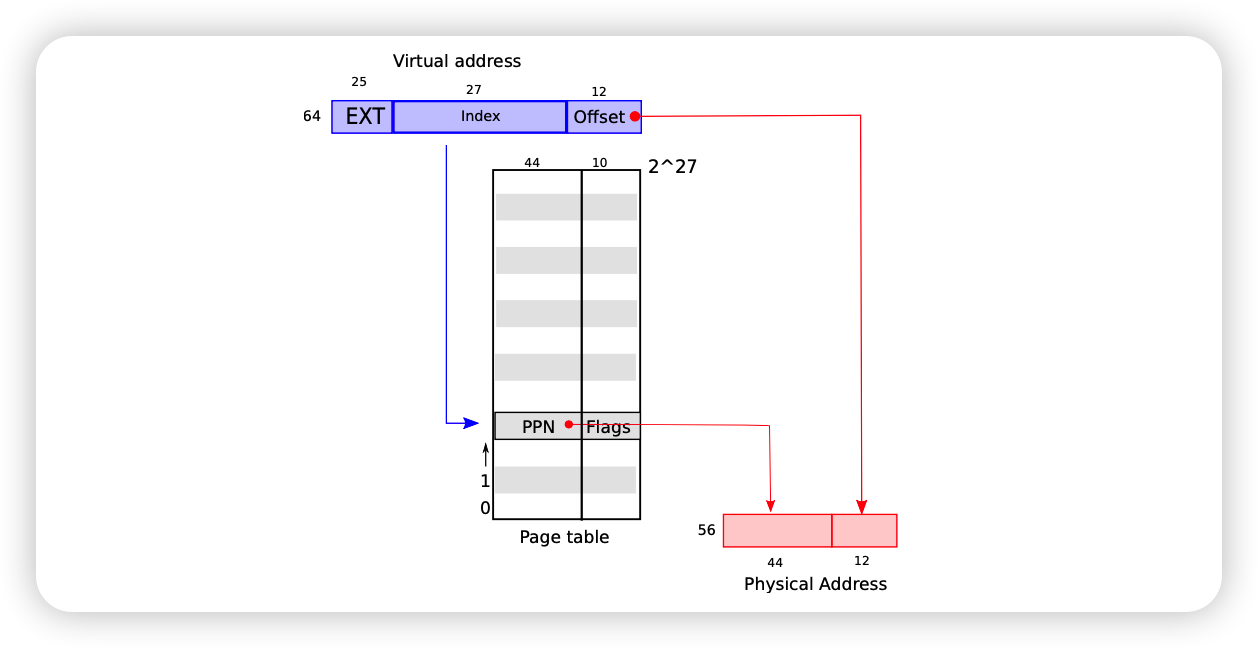
\includegraphics[width=0.8\textwidth]{../imgs/f3-1.png}
    \caption{RISC-V虚拟和物理地址(简化的逻辑页表)}
    \label{f3-1}
\end{figure}

\begin{figure}[htbp]
    \centering
    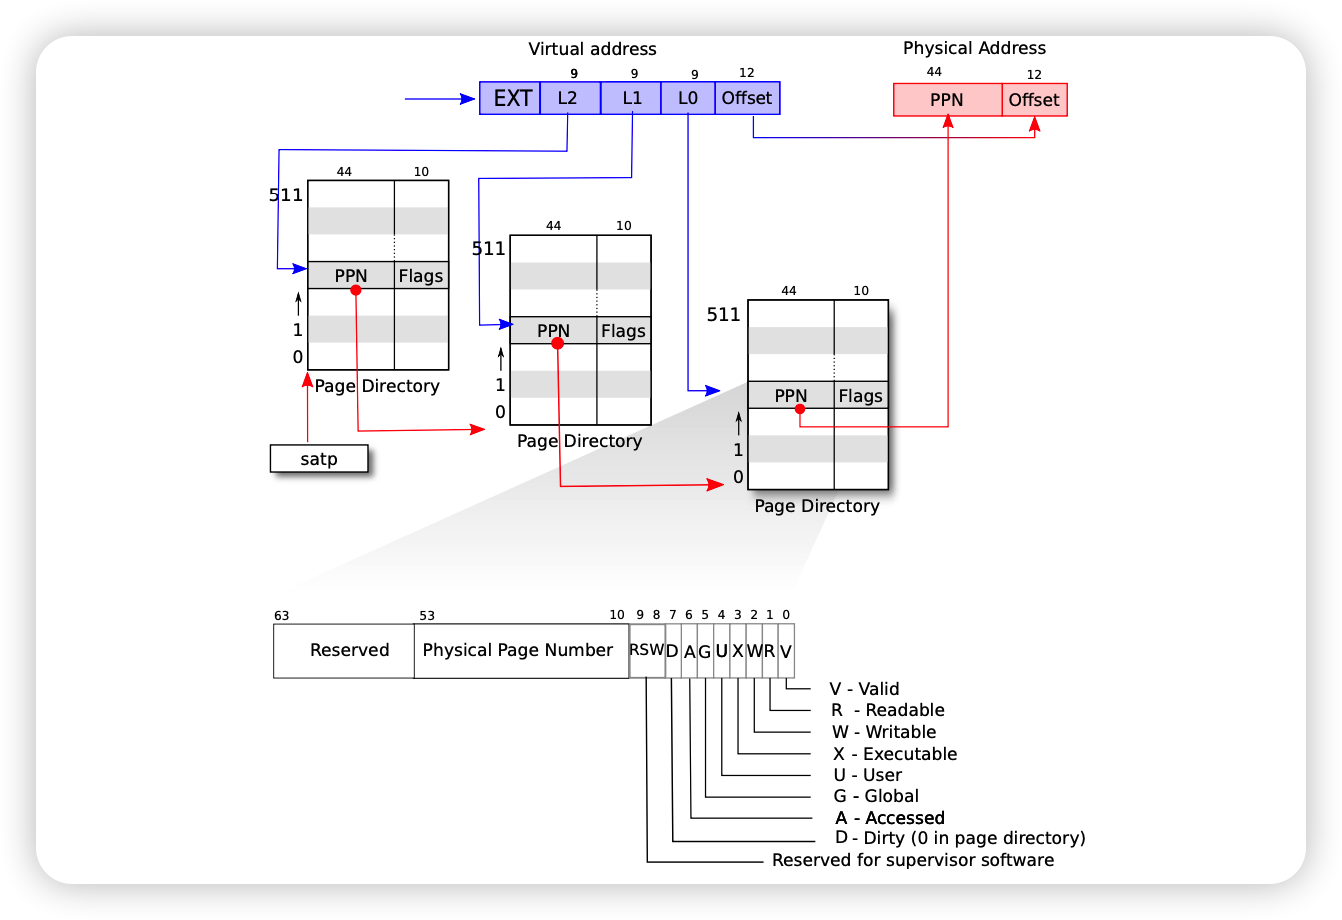
\includegraphics[width=0.8\textwidth]{../imgs/f3-2.png}
    \caption{RISC-V地址翻译细节}
    \label{f3-2}
\end{figure}

在Sv39 RISC-V中,虚拟地址的高25位不用于翻译。
物理地址也还有增长的空间:PTE的格式中还有空间可以让物理页号再增长10位。
RISC-V的设计者根据技术预测选择了这些数字。
$2^{39}$个字节也就是512GB的虚拟地址空间对于运行在RISC-V计算机中的应用来说应该足够了。
$2^{56}$的物理地址空间在不久的未来都足够容纳很多I/O设备和DRAM芯片。
如果还需要更大的空间,RISC-V的设计者还定义了48位虚拟地址的Sv48[3]。

如\autoref{f3-2}所示,一个RISC-V CPU用3步把一个虚拟地址翻译成物理地址。
页表以3级树的形式被存储在物理内存中。
树的根是一个4096字节的页表,它包含512个PTE,每个PTE中都包含了一个下一级页表的物理地址。
每个第二级页表都包含了512个PTE,每个PTE中都包含了树的最后一级。
分页硬件使用27位中的最高9位在根页表中选择一个PTE,用中间9位在第二级页表中选择一个PTE,用低9位去选择最终的PTE。(在Sv48 RISC-V中一个页表有4级,虚拟地址的第39到47位用来在顶级页表索引。)

如果翻译地址所需的三个PTE中的任何一个不存在,分页硬件会抛出一个\emph{页面错误异常(page-fault exception)},让内核来处理这个异常(见\autoref{ch04})。

\autoref{f3-2}中的3级架构与\autoref{f3-1}中的单级设计相比,可以用一种更加内存高效地方式记录PTE。
在通常情况下很大范围内的虚拟地址都没有映射,三级结构可以省略整个页面目录。
例如,如果一个应用只使用了从0开始的很少的页,那么顶级页表的1到511号表项都是无效的,因此kernel不需要为511个中间的页表分配页面。
因此,在这个例子中,3级的设计节省了511个中间的页表和$511 \times 512$个底级页表。

虽然CPU在执行load/store指令时在硬件中运行三级结构,但这种3级架构的一个潜在缺点是在执行load/store指令时CPU必须从内存中加载3个PTE才能把虚拟地址翻译到物理地址。
为了避免从物理内存中加载PTE的开销,RISC-V CPU会把页表项缓存在\emph{翻译查找缓冲区(Translation Look-aside Buffer, TLB)}中。

每个PTE都包含一些标注位,它们告诉分页硬件该虚拟地址允许的操作。
\texttt{PTE\_V}指示PTE是否存在:如果该位未被设置,那么引用对应的页面会导致异常(即不允许)。
\texttt{PTE\_R}控制指令是否可以读取该页。
\texttt{PTE\_W}控制指令是否可以写入该页。
\texttt{PTE\_X}控制指令是否可以把页的内容解释为指令并执行它们。
\texttt{PTE\_U}控制用户模式下的指令是否可以访问该页;如果\texttt{PTE\_U}未被设置,该PTE只能在管理模式下使用。
\autoref{f3-2}展示了所有这些位的含义。
这些标记和所有其他分页硬件相关的结构体定义在\href{https://github.com/mit-pdos/xv6-riscv/blob/riscv//kernel/riscv.h}{(kernel/riscv.h)}。

为了让CPU使用页表,内核必须把根页表的物理地址写入\texttt{satp}寄存器。
执行后续的指令时CPU会使用\texttt{satp}指向的页表来翻译所有的地址。
每个CPU都有自己的\texttt{satp},所以不同的CPU可以运行不同的进程,每个进程都有自己的页表所描述的地址空间。

通常内核会把所有物理内存都映射进页表里,这样它可以使用load/store指令读取和写入任何物理内存位置。
因为页面目录也在物理内存中,内核可以通过使用标准store指令写入PTE的虚拟地址来编程页面目录中PTE的内容。

解释一下相关的术语。
物理内存是指DRAM的存储单元。
物理内存中的每个字节都有一个地址,称为物理地址。
指令只使用虚拟地址,分页硬件把它翻译成物理地址,然后发送给DRAM硬件以读取或写入存储。
与物理内存和虚拟地址不同,虚拟内存并不是一个物理对象,而是指内核提供的管理物理内存和虚拟地址的抽象和机制的集合。

\section{内核地址空间}


